\section{Preprocessing}
\todo{Why did we do this?}

\subsection{E-Mail Parsing}
\todo{This is our simple technique}
\todo{
    \begin{itemize}
        \item Strip metadata
        \item Strip HTML
        \item Multipart Splitting
    \end{itemize}
}
\todo{Improvement?}

\subsection{Stemming}
\todo{Our first advanced techinque}

\todo{Improvement?}

\subsection{Feature selection}
\todo{Is this really preprocessing?}

As the number of features generated by the input data is even very high after the previous preprocessing steps, we are going to minimise its number by trimming features which are (siginificantly) relevant for the classification quality.

\todo{\dots}

\begin{figure}[h!]
    \centering
    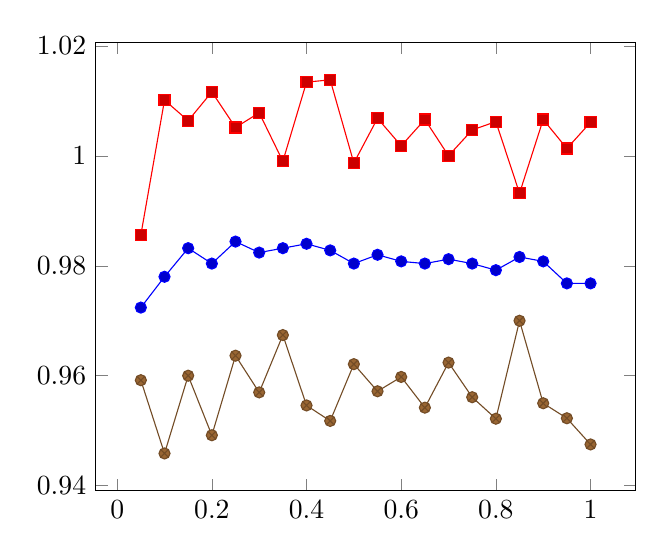
\begin{tikzpicture}
        \begin{axis}
             \addplot+[sharp plot] coordinates {
                (0.05, 0.972400)
                (0.10, 0.978000)
                (0.15, 0.983200)
                (0.20, 0.980400)
                (0.25, 0.984400)
                (0.30, 0.982400)
                (0.35, 0.983200)
                (0.40, 0.984000)
                (0.45, 0.982800)
                (0.50, 0.980400)
                (0.55, 0.982000)
                (0.60, 0.980800)
                (0.65, 0.980400)
                (0.70, 0.981200)
                (0.75, 0.980400)
                (0.80, 0.979200)
                (0.85, 0.981600)
                (0.90, 0.980800)
                (0.95, 0.976800)
                (1.00, 0.976800)
                };
             \addplot+[sharp plot] coordinates {
                (0.05, 0.972400+0.013206)
                (0.10, 0.978000+0.032125)
                (0.15, 0.983200+0.023186)
                (0.20, 0.980400+0.031215)
                (0.25, 0.984400+0.020746)
                (0.30, 0.982400+0.025424)
                (0.35, 0.983200+0.015799)
                (0.40, 0.984000+0.029394)
                (0.45, 0.982800+0.031010)
                (0.50, 0.980400+0.018287)
                (0.55, 0.982000+0.024819)
                (0.60, 0.980800+0.021014)
                (0.65, 0.980400+0.026199)
                (0.70, 0.981200+0.018804)
                (0.75, 0.980400+0.024298)
                (0.80, 0.979200+0.027011)
                (0.85, 0.981600+0.011593)
                (0.90, 0.980800+0.025799)
                (0.95, 0.976800+0.024528)
                (1.00, 0.976800+0.029285)
                };
             \addplot+[sharp plot] coordinates {
                (0.05, 0.972400-0.013206)
                (0.10, 0.978000-0.032125)
                (0.15, 0.983200-0.023186)
                (0.20, 0.980400-0.031215)
                (0.25, 0.984400-0.020746)
                (0.30, 0.982400-0.025424)
                (0.35, 0.983200-0.015799)
                (0.40, 0.984000-0.029394)
                (0.45, 0.982800-0.031010)
                (0.50, 0.980400-0.018287)
                (0.55, 0.982000-0.024819)
                (0.60, 0.980800-0.021014)
                (0.65, 0.980400-0.026199)
                (0.70, 0.981200-0.018804)
                (0.75, 0.980400-0.024298)
                (0.80, 0.979200-0.027011)
                (0.85, 0.981600-0.011593)
                (0.90, 0.980800-0.025799)
                (0.95, 0.976800-0.024528)
                (1.00, 0.976800-0.029285)
                };
    \end{axis}
    \end{tikzpicture}
    \caption{Accuracy w.r.t. upper threshold (lower threshold = 0)}
    \label{p:upperbound}
\end{figure}




\todo{Improvement?}

